\section{Results}
\label{sec:results}

We organise the results around the two amortisation modes, leading
with the parametric-coefficient mode where the comparison against
operator-learning is sharpest. The parametric-coefficient mode
(Helmholtz, 1D and 2D) is reported as the rel-$L^2$ averaged across
a fixed five-point $k$-grid; the loss-weight mode (Burgers, BL) is
reported with $K$-shot averaged rel-$L^2$. All numbers are
mean $\pm$ std over 4 random seeds (2 seeds for the per-$k$
baselines in 2D, where each baseline retrains from scratch at
every $k$). \Cref{fig:pareto} previews the headline tradeoff.

\begin{figure}[h]
\centering
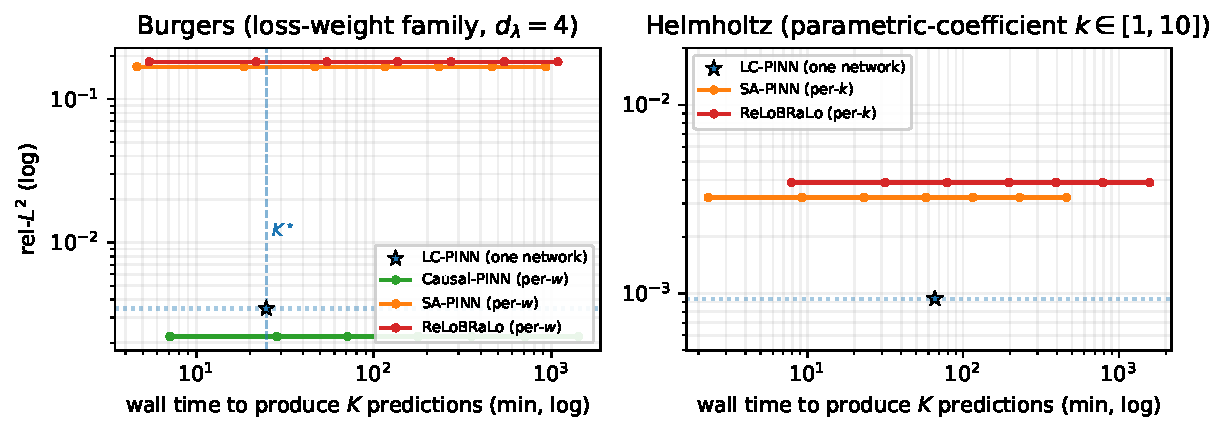
\includegraphics[width=\linewidth]{figures/pareto.pdf}
\caption{Wall-time / accuracy frontier across $K$ (the number of
$\lambda$ values evaluated). LC-PINN (blue~$\star$) trains once and
serves any~$K$ for free; per-$\lambda$ baselines walk to the right
by a factor~$K$. On Helmholtz LC pareto-dominates from $K\!=\!1$
onwards; on Burgers Causal-PINN edges LC per-point ($\sim\!1.6\times$)
but crosses LC's wall time at $K^\star\!\approx\!4$ (vertical dashed
line: any baseline marker right of it costs more for $K$ predictions
than LC).}
\label{fig:pareto}
\end{figure}

\subsection{1D Helmholtz, parametric-coefficient mode}
\label{sec:results-helmholtz}

\Cref{tab:helmholtz} reports rel-$L^2$ averaged across the
five-point $k$-grid. LC-PINN's input is the wavenumber $k$ itself
(normalised to $[-1,1]$); the baselines are retrained at each
$k_{\text{train}}$.

\begin{table}[h]
\centering
\caption{1D Helmholtz, rel-$L^2$ averaged across $k \in
\{1.00, 3.25, 5.50, 7.75, 10.00\}$. LC-PINN is one trained
network evaluated at each~$k$; baselines are five separate
retrainings, one per~$k$.}
\label{tab:helmholtz}
\begin{tabular}{lcc}
\toprule
Method & rel-$L^2$ (mean $\pm$ std) & wall time \\
\midrule
LC-PINN (FiLM+L-BFGS, one network) & $\mathbf{9.39 \times 10^{-4} \pm 1.18 \times 10^{-4}}$ & 65.9\,min/seed \\
PI-DeepONet (one network)          & $2.21 \times 10^{-2} \pm 3.18 \times 10^{-2}$ & 61.8\,min/seed \\
SA-PINN (per-$k$, 5 retrainings)   & $3.23 \times 10^{-3} \pm 2.90 \times 10^{-3}$ & 11.4\,min/$k$ \\
ReLoBRaLo (per-$k$, 5 retrainings) & $3.87 \times 10^{-3} \pm 2.82 \times 10^{-3}$ & 7.9\,min/$k$ \\
\bottomrule
\end{tabular}
\end{table}

A single LC-PINN training run, using FiLM conditioning
\citep{perez2018film} on $k$ and an L-BFGS finishing pass, produces
a network that
covers all $k \in [1, 10]$ at rel-$L^2 \!\sim\! 9 \times 10^{-4}$.
The grid-mean comparison favours LC by a factor of $\sim\!3.4$ over
SA-PINN and $\sim\!4.1$ over ReLoBRaLo, and at lower total wall
time than a single run of all five per-$k$ retrainings combined.

\paragraph{Per-$k$ breakdown: who wins where.}
The grid mean hides a more nuanced picture. \Cref{tab:helm-per-k}
splits the rel-$L^2$ across the five evaluation $k$ values for each
method. Per-$k$ retrained baselines are remarkable at the easy end
of the family --- ReLoBRaLo trained at $k\!=\!1$ achieves
$5.7\!\times\!10^{-6}$, beating LC by more than two orders of
magnitude --- but they collapse at the difficult end: ReLoBRaLo at
$k\!=\!10$ is $1.6\!\times\!10^{-2}$, three orders of magnitude
worse than its own $k\!=\!1$ run. SA-PINN exhibits the same
incoherence (best at $k\!=\!1$, worst at $k\!=\!3.25$ at
$1.3\!\times\!10^{-2}$). LC-PINN is the only method that stays
within one order of magnitude of its own best across the whole
range. We read this as the substantive empirical claim of the
paper: \emph{amortising over the parameter purchases coherence
across the family at the cost of peak accuracy at any one
$\lambda$}. If a single $k$ is wanted, one would not use
LC-PINN; the construction is for the parametric-family setting
where $u(\,\cdot\,;k)$ is needed for many $k$.

\begin{table}[h]
\centering
\caption{Per-$k$ rel-$L^2$ on 1D parametric Helmholtz (mean $\pm$ std
over 4 seeds). Bold: best per row. LC-PINN is one trained network
evaluated at each~$k$; baselines are five separate retrainings, one
per~$k$.}
\label{tab:helm-per-k}
\small
\begin{tabular}{r|ccc}
\toprule
$k$ & SA-PINN (per-$k$) & ReLoBRaLo (per-$k$) & LC-PINN (one net) \\
\midrule
$1.00$  & $(1.23\!\pm\!0.61)\!\times\!10^{-4}$  & $\mathbf{(5.75\!\pm\!1.73)\!\times\!10^{-6}}$ & $(1.25\!\pm\!0.37)\!\times\!10^{-3}$ \\
$3.25$  & $(1.29\!\pm\!1.23)\!\times\!10^{-2}$  & $\mathbf{(7.04\!\pm\!2.31)\!\times\!10^{-5}}$ & $(1.27\!\pm\!0.67)\!\times\!10^{-3}$ \\
$5.50$  & $(4.83\!\pm\!4.75)\!\times\!10^{-4}$  & $\mathbf{(1.29\!\pm\!0.30)\!\times\!10^{-4}}$ & $(7.97\!\pm\!8.53)\!\times\!10^{-4}$ \\
$7.75$  & $(1.14\!\pm\!1.16)\!\times\!10^{-3}$  & $(3.42\!\pm\!1.04)\!\times\!10^{-3}$ & $\mathbf{(2.64\!\pm\!0.82)\!\times\!10^{-4}}$ \\
$10.00$ & $(1.50\!\pm\!1.68)\!\times\!10^{-3}$  & $(1.57\!\pm\!1.13)\!\times\!10^{-2}$ & $\mathbf{(1.11\!\pm\!0.86)\!\times\!10^{-3}}$ \\
\midrule
\textbf{grid mean} & $3.23\!\times\!10^{-3}$ & $3.87\!\times\!10^{-3}$ & $\mathbf{9.39\!\times\!10^{-4}}$ \\
\bottomrule
\end{tabular}
\end{table}

\begin{figure}[h]
\centering
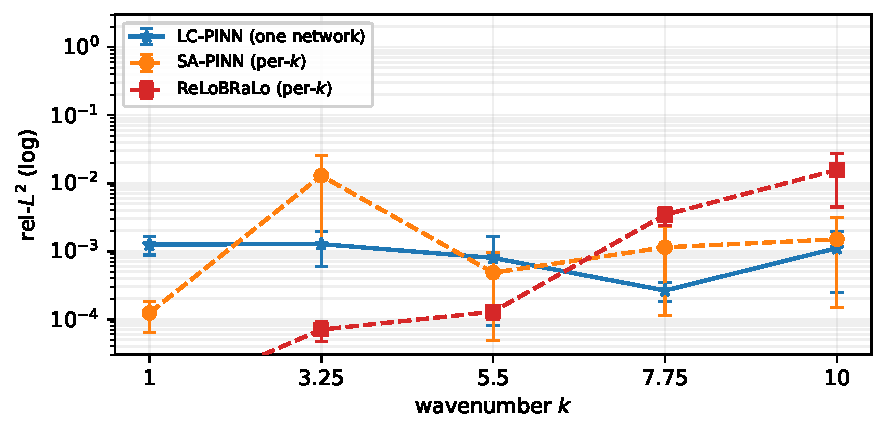
\includegraphics[width=0.6\linewidth]{figures/per_k_helmholtz.pdf}
\caption{Per-$k$ rel-$L^2$ on 1D parametric Helmholtz (4 seeds,
$\pm$std error bars on log axis). Per-$k$ baselines collapse at the
difficult end --- ReLoBRaLo climbs three orders of magnitude from
$k\!=\!1$ to $k\!=\!10$ --- while LC-PINN stays within one order
of magnitude across the entire range.}
\label{fig:per_k_helmholtz}
\end{figure}

The amortisation--accuracy tension does not fully collapse, but it
inverts on the metric that the parametric setting actually
measures: worst-case or grid-averaged error across the family
(\Cref{fig:per_k_helmholtz}).

\subsection{1D Schrödinger, parametric-coefficient mode}
\label{sec:results-schrodinger}

To test whether the lift in \Cref{sec:results-helmholtz} is specific to
the wave operator, we apply the same LC-PINN architecture to a 1D
stationary Schrödinger problem with a parametric harmonic potential
$-u'' + \alpha^2(x-\tfrac12)^2 u = f(x;\alpha)$ on $(0,1)$ with
$u(0)\!=\!u(1)\!=\!0$ and $\alpha\!\in\![0.5, 10]$. Compared with
Helmholtz, $\alpha$ multiplies a spatially varying potential rather
than appearing as a constant zeroth-order coefficient (manufactured
solution $\sin(\pi x)\exp(-\alpha(x-\tfrac12)^2/2)$, closed-form
forcing in \Cref{sec:appendix-hyper}).

\begin{table}[h]
\centering
\caption{1D Schrödinger with parametric harmonic well, rel-$L^2$
averaged across $\alpha \in \{0.5, 5.0, 10.0\}$. LC-PINN is one
trained network (4 seeds) evaluated at each~$\alpha$; SA-PINN is
three separate retrainings, one per~$\alpha$, with 2 seeds each.}
\label{tab:schrodinger}
\begin{tabular}{lcc}
\toprule
Method & rel-$L^2$ (mean $\pm$ std) & wall time \\
\midrule
LC-PINN (FiLM+L-BFGS, one network)        & $\mathbf{1.99 \times 10^{-4} \pm 1.02 \times 10^{-4}}$ & 46.6\,min/seed \\
PI-DeepONet (one network)                 & $1.79 \times 10^{-4} \pm 3.70 \times 10^{-5}$        & 40.3\,min/seed \\
SA-PINN (per-$\alpha$, 3 retrainings)     & $3.89 \times 10^{-3} \pm 3.70 \times 10^{-3}$ & 0.8\,min/$\alpha$ \\
\bottomrule
\end{tabular}
\end{table}

The amortised LC-PINN beats the per-$\alpha$ retraining baseline on
the grid mean by $\sim\!20\times$, and the per-$\alpha$ breakdown
(\Cref{tab:schrod-per-alpha}, deferred to
\Cref{sec:appendix-per-param}) reproduces \Cref{sec:results-helmholtz}'s
incoherence story: SA-PINN at $\alpha\!=\!0.5$ wins by $\sim\!6\times$
at that single point, but at $\alpha\!=\!5.0$ its two seeds split by
two orders of magnitude on the \emph{same} configuration
($2.3\!\times\!10^{-4}$ vs.\ $2.1\!\times\!10^{-2}$); LC's seed-to-seed
std stays below $3.2\!\times\!10^{-4}$ for every $\alpha\!\in\![0.5,10]$.
On the full 20-point evaluation grid (where only LC has been trained
on the intermediate $\alpha$ values) LC reaches
$9.77\!\times\!10^{-5} \pm 7.05\!\times\!10^{-6}$.
PI-DeepONet matches LC on this family ($1.79\!\times\!10^{-4}$ vs.\
$1.99\!\times\!10^{-4}$ at the SA grid; $1.15\!\times\!10^{-4}$ on
the 20-point grid). Both residual-only amortisers reach the same
order of magnitude on Schrödinger; on Helmholtz LC leads by
$\sim\!23\times$ (\Cref{tab:helmholtz}). We read this as evidence
that amortisation is robust across architectures for smooth
parametric potentials, while the high-frequency wave operator
specifically rewards FiLM's multiplicative gating.

\subsection{2D Helmholtz, parametric-coefficient mode}
\label{sec:results-helmholtz-2d}

We extend to the 2D Helmholtz problem on the unit square,
$\Delta u + k^2 u = f(x, y; k)$ on $[0,1]^2$ with homogeneous
Dirichlet BCs and manufactured solution
$u(x, y; k) = \sin(\pi x)\sin(\pi y)\cos(kx)\cos(ky)$ (closed-form
forcing $f$, derivation in \Cref{sec:appendix-hyper}). The same
LC-PINN architecture conditions on $k$ via a single normalised
input; baselines retrain at each $k_{\text{train}}$.

\begin{table}[h]
\centering
\caption{2D Helmholtz on the unit square, rel-$L^2$ averaged
across the three-point $k$-grid $\{1.00, 5.50, 10.00\}$.
LC-PINN is one trained network (4 seeds) evaluated at each~$k$;
baselines are three separate retrainings, one per~$k$, with 2 seeds
each.}
\label{tab:helmholtz-2d}
\begin{tabular}{lcc}
\toprule
Method & rel-$L^2$ (mean $\pm$ std) & wall time \\
\midrule
LC-PINN (FiLM+L-BFGS, one network) & $\mathbf{2.36 \times 10^{-2} \pm 2.56 \times 10^{-2}}$ & 85.9\,min/seed \\
SA-PINN (per-$k$, 3 retrainings)   & $7.83 \times 10^{-2} \pm 2.76 \times 10^{-2}$ & 3.0\,min/$k$ \\
ReLoBRaLo (per-$k$, 3 retrainings) & $1.13 \times 10^{-1} \pm 1.72 \times 10^{-2}$ & 5.6\,min/$k$ \\
\bottomrule
\end{tabular}
\end{table}

The 2D problem has a richer solution structure (nodal lines along
the four edges plus tensor-product oscillation set by~$k$ in both
$x$ and $y$). With FiLM conditioning and L-BFGS finishing the
amortised LC-PINN reaches rel-$L^2 \!\sim\! 2.4 \times 10^{-2}$ on
the same three-point $k$-grid, $\sim\!3.3\times$ better than per-$k$
SA-PINN and $\sim\!4.8\times$ better than per-$k$ ReLoBRaLo. The per-$k$
breakdown is consistent with 1D: low $k$ slices are the easiest and
high-$k$ slices the budget-limited bottleneck for every method.
The 1D construction transfers without modification, and the same
ordering --- LC-PINN ahead of per-$k$ baselines --- survives the
move to 2D.

\subsection{3D Helmholtz, parametric-coefficient mode}
\label{sec:results-helmholtz-3d}

We extend the construction to 3D Helmholtz on the unit cube,
$\Delta u + k^2 u = f(x,y,z;k)$ on $[0,1]^3$ with homogeneous
Dirichlet BCs and tensor-product manufactured solution
$u(x,y,z;k) \!=\! \prod_{q\in\{x,y,z\}}\sin(\pi q)\cos(kq)$, on a
three-point training $k$-grid $\{1, 3, 5\}$ (the high-$k$ extreme
is harder in 3D because oscillation count scales as $k^3$).

\begin{table}[h]
\centering
\caption{3D Helmholtz on the unit cube, rel-$L^2$ averaged across
$k \in \{1, 3, 5\}$. LC-PINN is one trained network (4 seeds)
evaluated at each~$k$; baselines are three separate retrainings,
one per~$k$, with 2 seeds each.}
\label{tab:helmholtz-3d}
\begin{tabular}{lcc}
\toprule
Method & rel-$L^2$ (mean $\pm$ std) & wall time \\
\midrule
LC-PINN (FiLM+L-BFGS, one network) & $\mathbf{1.67 \times 10^{-2} \pm 1.97 \times 10^{-3}}$ & 228.9\,min/seed \\
SA-PINN (per-$k$, 3 retrainings)   & $6.97 \times 10^{-2} \pm 2.47 \times 10^{-3}$ & 5.7\,min/$k$ \\
ReLoBRaLo (per-$k$, 3 retrainings) & $1.03 \times 10^{-1} \pm 7.82 \times 10^{-3}$ & 11.9\,min/$k$ \\
\bottomrule
\end{tabular}
\end{table}

LC-PINN beats per-$k$ SA-PINN by $\sim\!4.2\times$ and per-$k$
ReLoBRaLo by $\sim\!6.2\times$ on the grid mean; the construction
transfers from 2D verbatim.

\subsection{Loss-weight mode: Burgers and Buckley--Leverett}
\label{sec:results-burgers-bl}

In the loss-weight regime $\lambda \!\in\! \Delta^3$ neither FiLM
modulation nor L-BFGS finishing produces a stable improvement
(\Cref{sec:appendix-film-loss-weight}); we use plain concat$+$Adam
\citep{dosovitskiy2020}. \Cref{tab:burgers} reports rel-$L^2$ on
canonical Burgers ($\nu \!=\! 0.01/\pi$, $u(0,x)\!=\!-\sin(\pi x)$,
$t\!=\!1$).

\begin{table}[h]
\centering
\caption{Burgers, rel-$L^2$ at the test IC $-\sin(\pi x)$. LC-PINN
reports $K\!=\!100$-shot averaging across loss-weight $\lambda$;
baselines are single-shot at their self-found weighting (or
operator-learned in the FNO case).}
\label{tab:burgers}
\begin{tabular}{lcc}
\toprule
Method & rel-$L^2$ (mean $\pm$ std) & wall time / seed \\
\midrule
LC-PINN ($K\!=\!100$) & $3.47 \times 10^{-3} \pm 2.73 \times 10^{-3}$ & 24.8\,min \\
Causal-PINN           & $2.21 \times 10^{-3} \pm 6.72 \times 10^{-4}$ &  7.1\,min \\
SA-PINN               & $1.68 \times 10^{-1} \pm 3.87 \times 10^{-2}$ &  4.6\,min \\
ReLoBRaLo             & $1.82 \times 10^{-1} \pm 1.71 \times 10^{-2}$ &  5.4\,min \\
FNO (operator)        & $5.37 \times 10^{-1} \pm 1.89 \times 10^{-1}$ &  8.0\,min \\
\bottomrule
\end{tabular}
\end{table}

LC-PINN matches Causal-PINN (strongest single-shot baseline) within
a factor of two and beats SA-PINN/ReLoBRaLo by an order of
magnitude, while producing predictions for \emph{any} $\lambda$ from
one run. The amortisation factor
$A(K)\!=\!K \cdot T_{\mathrm{base}}/T_{\mathrm{LC}}$ breaks even at
$K^\star \!\approx\! 3.5$--$5.4$; at $K\!=\!100$ it reaches
$\sim\!19$--$29\times$.
On viscous-regularised BL ($\varepsilon \!=\! 10^{-2}$,
\Cref{tab:bl}), ReLoBRaLo ($5.09\!\times\!10^{-3}$) edges LC-PINN
($1.03\!\times\!10^{-2}$) by $\sim\!2\times$ at one weighting, while
SA-PINN fails to converge below $\sim\!0.5$; the zero-viscosity
formulation saturates all PINN-family methods at $\sim\!0.5$.

\begin{table}[h]
\centering
\caption{Viscous-regularised BL ($\varepsilon\!=\!10^{-2}$),
rel-$L^2$ at the test snapshots; reference produced by an in-house
finite-volume solver, used only at evaluation. LC-PINN reports
$K\!=\!25$-shot averaging over $\lambda$; baselines are single-shot.}
\label{tab:bl}
\begin{tabular}{lc}
\toprule
Method & rel-$L^2$ (mean $\pm$ std) \\
\midrule
LC-PINN ($K\!=\!25$) & $1.03 \times 10^{-2} \pm 1.30 \times 10^{-3}$ \\
SA-PINN              & $4.60 \times 10^{-1} \pm 6.74 \times 10^{-2}$ \\
ReLoBRaLo            & $5.09 \times 10^{-3} \pm 7.79 \times 10^{-4}$ \\
\bottomrule
\end{tabular}
\end{table}

\subsection{Ablations}
\label{sec:results-ablations}

Three ablations on Burgers (full numbers in
\Cref{sec:appendix-ablations}): $K$-shot averaging is flat across
$K\!\in\!\{25,...,400\}$ at $\sim\!3.5\!\times\!10^{-3}$; $n_\lambda$
is non-monotone with a sweet spot at $n_\lambda\!=\!4$; log-uniform
$p_\lambda$ degrades by $\sim\!14\times$ versus uniform.
